\chapter{Strontium Rydberg Experiment}
\label{ch:experiment}

This chapter describes the Rydberg apparatus used in this work.
It provides documentation of the current state of various systems for producing ultracold and quantum degenerate gases of strontium. 
Being the third ultracold strontium at Rice, we were able to leverage lessons learned on the previous experiments (generally referred to as ``Neutral'' and ``Plasma'') to build build quite a capable and flexible system.

Although most of our system looks very similar to other ultracold strontium systems, what makes our system different is the inclusion of systems for creating, manipulating, and detecting charged particles. 
In particular, we have in-vacuum electric field plates to cancel stray electric fields as well as ramp to ionizing fields which direct electrons or ions towards the microchannel plate (MCP) detector.

Our old-school ``metal can'' setup can't compete with the optical access provided by many recently started alkaline-earth Rydberg tweezer systems using glass cells \cite{Norcia2018.PRX.8.041054, Cooper2018.PRX.8.041055, Saskin2019.PRL.122.143002}.
There's still a place for our system which likely provides capabilities for better shielding from stray electric fields, performing SFI, and the ability to detect charged particles which, without going to significantly custom systems, are somewhat limiting on the standard glass cell setups.

\section{Producing Cold and Ultracold Gases of Strontium}

We follow the standard laser cooling and trapping sequence for producing cold and ultracold gases of strontium.
Detailed explanations of the techniques are available from various sources (e.g., \cite{Boyd2007.PhD, Stellmer2013.PRA.87.013611, Mickelson2010.PhD, Martinez2012.PhD, Stellmer2013.PhD, Barker2016.PhD}) so the process will only be outlined here for context.

\subsection{Pre-cooling on the $\SI{461}{\nm}$ Transition}

Due to strontium's low vapor pressure, an oven is required to sublimate strontium in to a gaseous form.
Our strontium oven operates at about $\SI{425}{\celsius}$ with the nozzle at about $\SI{390}{\celsius}$\footnote{Ideally the nozzle should be hotter than the oven to reduce the chances of clogging but it's likely that our actual oven temperature is a bit lower due to the temperature sensor being buried in the oven's heating element rather than in the oven itself.}.
Other strontium experiments typically run their ovens between $\SIrange[range-phrase=-]{450}{650}{\celsius}$\footnote{$\SI{450}{\celsius}$ \cite{Schioppo2012.RSI.83.103101}, $\SI{500}{\celsius}$ \cite{Campbell2017.PhD}, $\SI{575}{\celsius}$ (body) and $\SI{850}{\celsius}$ (nozzle) \cite{Boyd2007.PhD, Ludlow2008.PhD}, $\SI{600}{\celsius}$ (reservoir) and $\SI{650}{\celsius}$ (nozzle) \cite{Barker2016.PhD, Senaratne2018.PhD}, $\SIrange[range-phrase=-]{600}{750}{\celsius}$ \cite{Stellmer2013.PhD, Stellmer2013.PRA.87.013611}.} so we have some headroom to increase the oven temperature and increase the strontium flux\footnote{Although this could possibly degrade our trap lifetime.}.
See \cref{ssec:source-side_vacuum} for more details about our strontium oven.

Immediately after the atoms exit the oven, they pass through the two-dimensional (2D) collimator stage which applies transverse optical molasses \cite{Balykin1984.JETP.63.508, Balykin1985.JOSAB.2.1776, Lett1989.JOSAB.6.2084, Joffe1993.JOSAB.10.2257, Hoogerland1996.APB.62.323} to reduce the divergence of the atomic beam.
The $\SI{461}{\nm}$ $\nSLJ{5s^2}{1}{S}{0} \rightarrow \nSLJ{5s5p}{1}{P}{1}$ transition is used because of the large $\flatfrac{\Gamma}{2\pi} = \SI{30.5}{\MHz}$ linewidth.
Some experiments have incorporated a 2D magneto-optical trap (MOT) which can not only focus the atomic beam but can also deflect the atoms so that only cold atoms enter the experiment region \cite{Yang2015.EPJD.69.226}\footnote{The designs presented in \cite{Dorscher2013.RSI.84.043109, Lamporesi2013.RSI.84.063102, Nosske2017.PRA.96.053415, Nosske2018.PRA.97.039901} are probably the more ``traditional'' 2D MOT which forms a cold line of atoms which are then ``pushed'' to the main chamber.}.
In order to maximize the efficiency of the 2D collimator, elliptical beams are used to increase the intensity along the atomic beam.

Since the 2D collimator has no effect on the longitudinal velocity, they atoms are still moving at about $v_{\text{avg}} \approx \SI{483}{\meter\per\second}$\footnote{Assuming the atomic beam leaves the oven at $T = \SI{425}{\celsius}$: $v_{\text{mp}} \approx \SI{445}{\meter\per\second}$, $v_{\text{avg}} \approx \SI{483}{\meter\per\second}$, and $v_{\text{rms}} \approx \SI{514}{\meter\per\second}$ \cite{Metcalf1999.LCT}.}, much too quickly to be trapped by a MOT operating on the $\SI{461}{\nm}$ transition which has a capture velocity of about $v_C \approx \SI{14}{\meter\per\second}$\footnote{The capture velocity defined as $v_C \equiv \flatfrac{\Gamma}{k}$ where $\Gamma$ is the transition linewidth and $k$ is the transition wavevector \cite{Metcalf1999.LCT}.} \cite{Camargo2015.MS, Metcalf1999.LCT}.
The atoms are slowed longitudinally with a Zeeman slower where a spatially-varying magnetic field keeps the atoms in resonance with a \SI{461}{\nm} beam counterpropagating their direction of travel \cite{Phillips1982.PRL.48.596}.
Because the  magnetic field is axial, a circularly polarized $\SI{461}{\nm}$ beam is used.
The atoms scatter about ** xxx photons ** which means they exit the Zeeman slower at about ** xxx m/s **.
Atoms moving faster than the ** design velocity of the Zeeman slower ** remain unaffected and continue through without being slowed.

***************

Isotope shift of the \SI{461}{\nm} transition.

\begin{table}[h]
	\caption{
		\label{tab:blue_isotope_shift}
		Isotope shifts of the $\SI{461}{\nm}$ $\nSLJ{5s^2}{1}{S}{0} \rightarrow \nSLJ{5s5p}{1}{P}{1}$ transition relative to \Sr{88}.
		Due to the hyperfine structure of \Sr{87}, the isotope shift is given relative to the center-of-gravity of the upper $\nSLJ{5s5p}{1}{P}{1}$ state.
		Transitions to a specific $\nSLJF{5s5p}{1}{P}{1}{F}$ state can be calculated with the $A$ and $B$ hyperfine constants in \cref{tab:hyperfine_coefficients_5s5p1P1}.}
	\centering
	\begin{tabular}{@{}ccccc@{}}
		\toprule
		Isotope						& Lower level								& Upper level								& $\nu - \nu_{88}$ [$\si{\MHz}$]	& Ref.								\\
		\midrule
		\Sr{88}						& $\nSLJ{5s^2}{1}{S}{0}$					& $\nSLJ{5s5p}{1}{P}{1}$					& $\num{0}$							&									\\
		\midrule
		\multirow{3}{*}{\Sr{87}}	& \multirow{3}{*}{$\nSLJ{5s^2}{1}{S}{0}$}	& \multirow{3}{*}{$\nSLJ{5s5p}{1}{P}{1}$}	& $\num{-46.3+-2.0}$				& \cite{Eliel1983.ZP.311.1}			\\
									&											& 											& $\num{-49.2+-3.6}$				& \cite{Buchinger1985.PRC.32.2058}	\\
									&											& 											& $\num{-44.6+-0.4}$				& \cite{Bushaw2000.SAPB.55.1679}	\\
		\midrule
		\multirow{3}{*}{\Sr{86}}	& \multirow{3}{*}{$\nSLJ{5s^2}{1}{S}{0}$}	& \multirow{3}{*}{$\nSLJ{5s5p}{1}{P}{1}$}	& $\num{-124.8+-0.3}$				& \cite{Eliel1983.ZP.311.1}			\\
									&											&											& $\num{-124.5+-1.3}$				& \cite{Buchinger1985.PRC.32.2058}	\\
									&											&											& $\num{-126.3+-0.2}$				& \cite{Bushaw2000.SAPB.55.1679}	\\
		\midrule
		\multirow{3}{*}{\Sr{84}}	& \multirow{3}{*}{$\nSLJ{5s^2}{1}{S}{0}$}	& \multirow{3}{*}{$\nSLJ{5s5p}{1}{P}{1}$}	& $\num{-270.8+-1.4}$				& \cite{Eliel1983.ZP.311.1}			\\
									&											&											& $\num{-270.6+-2.4}$				& \cite{Buchinger1985.PRC.32.2058}	\\
									&											&											& $\num{-273.2+-0.3}$				& \cite{Bushaw2000.SAPB.55.1679}	\\
		\bottomrule
	\end{tabular}
\end{table}

\begin{table}[h]
	\caption{
		\label{tab:hyperfine_coefficients_5s5p1P1}
		\Sr{87} hyperfine $A$ and $B$ coefficients for the $\nSLJ{5s5p}{1}{P}{1}$ state and calculated shifts from the center-of-gravity.}
	\centering
	\begin{tabular}{@{}cccccc@{}}
		\toprule
		$A$ [$\si{\MHz}$]						& $B$ [$\si{\MHz}$]						& Ref. 												& Lower level												& Upper level								& $\Delta E_{HF}$ [$\si{\MHz}$]	\\
		\midrule	
		\multirow{3}{*}{\num{-3.4+-0.4}}		& \multirow{3}{*}{\num{39+-4}}			& \multirow{3}{*}{\cite{Kluge1974.ZP.270.295}}		& \multirow{3}{*}{$\nSLJf{5s^2}{1}{S}{0}{\flatfrac{9}{2}}$}	& $\nSLJf{5s5p}{1}{P}{1}{\flatfrac{7}{2}}$	& $\num{36.6+-2.9}$				\\
												&										&													&															& $\nSLJf{5s5p}{1}{P}{1}{\flatfrac{11}{2}}$	& $\num{-5.5+-2.1}$				\\
												&										&													&															& $\nSLJf{5s5p}{1}{P}{1}{\flatfrac{9}{2}}$	& $\num{-22.6+-2.7}$			\\
		\midrule	
		\multirow{3}{*}{\num{-3.334+-0.025}}	& \multirow{3}{*}{\num{40.29+-0.21}}	& \multirow{3}{*}{\cite{Bushaw2000.SAPB.55.1679}}	& \multirow{3}{*}{$\nSLJf{5s^2}{1}{S}{0}{\flatfrac{9}{2}}$}	& $\nSLJf{5s5p}{1}{P}{1}{\flatfrac{7}{2}}$	& $\num{36.80+-0.17}$			\\
												&										&													&															& $\nSLJf{5s5p}{1}{P}{1}{\flatfrac{11}{2}}$	& $\num{-4.93+-0.12}$			\\
												&										&													&															& $\nSLJf{5s5p}{1}{P}{1}{\flatfrac{9}{2}}$	& $\num{-23.53+-0.14}$			\\
		\bottomrule
	\end{tabular}
\end{table}

\subsection{$\SI{461}{\nm}$ ``Blue'' MOT and Magnetic Trap}

Now that a significant portion of the atoms have been slowed by the Zeeman slower, they enter the main chamber where they are cooled and trapped by a standard six-beam $\SI{461}{\nm}$ ``blue'' MOT.
The MOT uses a quadrupole magnetic field and light detuned below atomic resonance to provide both position-dependent and velocity-dependent forces which captures and cools the atoms \cite{Raab1987.PRL.59.2631, Metcalf1999.LCT, Foot2005.Atomic}. 
Our blue MOT typically produces samples of atoms around $\SIrange[range-phrase=-]{1}{2}{\milli\kelvin}$.
Some experiments (e.g., \cite{Barker2016.PhD}) implement a ``cold MOT'' stage where detuning, intensity, and quadrupole gradient are ramped during the repumping process to obtain colder temperatures for the red MOT but we found that our temperatures are sufficient for decent transfer to the red MOT.

\begin{figure}[htbp]
	\includesvg[keepaspectratio, width=\textwidth, height=\textheight]{experiment/blue_system/old_blue_MOT.svg}
	\caption{\label{fig:old_blue_MOT}
		An early picture of our \Sr{88} blue MOT taken on 2014/08/29 through a \SI{2.75}{\inch} viewport with the atom source and Zeeman slower are off to the right.
		Considering the electric field plates are separated by about \SI{1}{\inch}, this blue MOT is likely has a diameter of about \SI{0.5}{\inch}. 
		A video is available at {https://youtu.be/ENDIizrlqMA}.}
\end{figure}

Although the $\SI{461}{\nm}$ is capable of scattering many photons per second, the Doppler limit of this transition is about $T_{D} = \SI{732}{\micro\kelvin}$\footnote{For the $\SI{461}{\nm}$ transition: $k_{B} T_{D} \equiv \flatfrac{\hbar \Gamma}{2} = \SI{732}{\micro\kelvin}$, $k_{B} T_{r} \equiv \flatfrac{\hbar^2 k^2}{2 M} = \SI{512}{\nano\kelvin}$.} \cite{Metcalf1999.LCT}.
Although sub-Doppler cooling is not available in the bosonic isotopes due to the lack of hyperfine structure, it has been observed in \Sr{87} where the blue MOT was measured to be about $\SI{300}{\micro\kelvin}$ \cite{Xu2003.PRL.90.193002, Xu2003.JOSAB.20.968}.
Interestingly, as noted in \cite{Xu2003.PRL.90.193002}, cooling bosonic alkaline-earth atoms on the $\SLJ{1}{S}{0} \rightarrow \SLJ{1}{P}{1}$ transition always seem to end up a few times the Doppler cooling limit until the intensity is close to zero \cite{Kisters1994.APB.59.89, Xu2002.PRA.66.011401, Xu2003.JOSAB.20.968}.

The $\SLJ{1}{S}{0} \rightarrow \SLJ{1}{P}{1}$ transition is not completely closed with about $\num{1} \colon \num{50000}$ decays following the $\nSLJ{5s5p}{1}{P}{1} \rightarrow \nSLJ{5s4d}{1}{D}{2}$ decay path.
About $\flatfrac{2}{3}$ then decay to the $\nSLJ{5s5p}{3}{P}{1}$ which then decays to the $\nSLJ{5s^2}{1}{S}{0}$ and return to the \SI{461}{\nm} cooling cycle.
The remaining $\flatfrac{1}{3}$ decay to the long-lived metastable $\nSLJ{5s5p}{3}{P}{2}$ states with lifetimes of about \SI{520}{\second} \cite{Yasuda2004.PRL.92.153004}, effectively removing them from the blue MOT cooling cycle.
Of the $\nSLJ{5s5p}{3}{P}{2}$ states, the low-field seeking $m_J = 1, 2$ states can become trapped in the quadrupole magnetic field of the blue MOT.
This decay path, initially seen as a loss from the blue MOT, ends up being a powerful tool for accumulating atoms in metastable reservoir \cite{Nagel2003.PRA.67.011401} at roughly the same temperature as the blue MOT. 
The magnetic trap was an essential tool in overcoming the abysmal $\SI{0.56(2)}{\percent}$ natural abundance of \Sr{84} to produce the first strontium BECs \cite{Stellmer2009.PRL.103.200401, Martinez2009.PRL.103.200402}.
** For details of our magnetic trap, see \cite{Camargo2015.MS}. **
The magnetic trap is also essential when loading multiple isotopes.
Since the isotope shift of the $\SI{461}{\nm}$ transition are comparable to the linewidth, it's difficult to simultaneously trap multiple isotopes. 
Trapping multiple isotopes is achieved through by sequentially operating a blue MOT tuned to different isotopes which loads the magnetic trap with the specific isotope before tuning the laser to another trap another isotope. 

Before moving on to the next cooling stage, atoms in the magnetic trap need to be recovered.
Several transitions have been explored for repumping atoms out of the metastable resevoir over the years (\cite{Stellmer2013.PhD} gives excellent descriptions in his thesis):
** I don't know if I want to keep the list below since it's very similar to one in Simon Stellmer's thesis **
\begin{itemize}
	\item {$\nSLJ{5s6s}{3}{S}{1}$} at $\SI{707}{\nm}$ --
		this is a popular transition and is used by a lot of past and current strontium experiments \cite{Courtillot2005.EPJD.33.161, Boyd2007.PhD, Ludlow2008.PhD, Barker2015.PRA.92.043418, Campbell2017.PhD, Cooper2018.PRX.8.041055, Norcia2018.PRX.8.041054} since it's well characterized and easily accessible with available laser diodes.
		The drawback is that this upper state is $J=1$ meaning $\nSLJ{5s6s}{3}{S}{1}$ can decay to the metastable $\nSLJ{5s5p}{3}{P}{0}$ state as well, requiring another laser at \SI{679}{\nm} to repump out of this state. 
	\item {$\nSLJ{5s4d}{3}{D}{2}$} --
		at $\SI{3011.84}{\nm}$ driving the $\nSLJ{5s5p}{3}{P}{2} \rightarrow \nSLJ{5s4d}{3}{D}{2}$ \cite{Mickelson2009.JPB.42.235001} transition.
		Being a $J=2$ state means a single laser can be used to clear out the $\nSLJ{5s5p}{3}{P}{2}$ reservoir but the \SI{3}{\um} wavelength is difficult to produce.
	\item {$\nSLJ{5s5d}{3}{D}{2}$} --
		at $\SI{496.93}{\nm}$ driving the $\nSLJ{5s5p}{3}{P}{2} \rightarrow \nSLJ{5s5d}{3}{D}{2}$ transition \cite{Stellmer2013.PhD, Stellmer2014.PRA.90.022512, Moriya2018.JPC.2.125008}.
		The challenge of using this transition is the difficulty in producing the green repumping light which typically requires frequency doubling (e.g., \cite{Mason2013.BS}).
	\item {$\nSLJ{5s6d}{3}{D}{1,2}$} --
		at $\SI{403.35}{\nm}$ driving the $\nSLJ{5s5p}{3}{P}{2} \rightarrow \nSLJ{5s6d}{3}{D}{2}$ transition \cite{Stellmer2014.PRA.90.022512, Moriya2018.JPC.2.125008}.
		Similar attributes as using the $\nSLJ{5s5d}{3}{D}{2}$ with the added advantage of being accessible with Blu-ray laser diodes.
	\item {$\nSLJ{5p^2}{3}{P}{1,2}$} --
		at $\SI{481.323}{\nm}$ driving the $\nSLJ{5s5p}{3}{P}{2} \rightarrow \nSLJ{5p^2}{3}{P}{2}$ transition \cite{Wongwaitayakornkul2013.BS, Camargo2015.MS, Ding2016.MS, Couturier2018.RSI.89.043103, Hu2019.PRA.99.033422}.
\end{itemize}
On our experiment, we use the $\SI{481}{\nm}$ transition.

\subsection{$\SI{689}{\nm}$ ``Red'' MOT}

After repumping, we further cool the sample by operating a MOT on the narrow ($\Gamma/2\pi = \SI{7.5}{\kHz}$) $\nSLJ{5s^2}{1}{S}{0} \rightarrow \nSLJ{5s5p}{3}{P}{1}$ transition at $\SI{689}{\nm}$ which has a Doppler limit of $T_{D} = \SI{180}{\nano\kelvin}$ and recoil limit of $T_{r} = \SI{229}{\nano\kelvin}$.
Following \cite{Loftus2004.PRA.70.063413}, MOTs can be characterized by the ratio of the transition linewidth ($\Gamma$) to the single photon recoil frequency shift ($\omega_R$) with typical MOTs operating in the regime $\flatfrac{\Gamma}{\omega_R} \gg 1$ compared to narrow line MOTs where $\flatfrac{\Gamma}{\omega_R} \sim 1$.
Operating in the $\flatfrac{\Gamma}{\omega_R} \sim 1$ regime where a few photon recoils can kick an atom out of resonance with the cooling lasers leads to very different dynamics.
The differences in dynamics are especially apparent in the shape of the bosonic red MOTs ** FIGURE? **. 
The fermionic red MOT may look similar to a $\flatfrac{\Gamma}{\omega_R} \gg 1$ MOT but it's shape is due to complications arising from hyperfine structure.
An excellent description of how the narrow $\SI{689}{\nm}$ ``red'' MOT works for both the bosons and fermion is presented in \cite{Stellmer2013.PhD}\footnote{Generally referred to as the ``Red MOT Bible''.} with additional resources in \cite{Boyd2007.PhD, Stellmer2014.arXiv.1307.0601}.

Considering first the bosonic case, the $\Gamma/2\pi = \SI{7.5}{\kHz}$ transition is a bit too narrow to effectively capture the $\sim \SI{2}{\milli\kelvin}$ atoms from the blue MOT.
In order to increase the transfer efficiency, the spectrum of the red MOT light is artifically broadened by frequency modulation, typically a few megahertz, which can be somewhat thought of as making the transition linewidth broader. 
Once enough atoms have been captured in the ``broadband'' red MOT, the frequency modulation and intensity is ramped down\footnote{Reducing the frequency modulation essentially increases the intensity of each comb tooth in the FM spectrum.} to a narrow or single-frequency red MOT where the coldest temperatures are achieved.

While the bosonic isotopes of strontium behave like an ideal $J=0 \rightarrow J=1$ MOT as described in texts (e.g., \cite{Metcalf1999.LCT, Foot2005.Atomic}) and are relatively straightforward to cool to sub-$\SI{2}{\micro\kelvin}$ temperatures, the hyperfine structure of \Sr{87} poses a unique challenge.
Since the ground state has (essentially) no magnetic moment, the position-dependent Zeeman shift is only experienced by the upper state but this results in the both a restoring force for some positions and transitions and an anti-traping force for other transitions and positions.
Narrow line laser cooling of \Sr{7} was first achieved by the Tokyo group where the uesd a ``trap'' laser resonant with the $\nSLJf{5s^2}{1}{S}{0}{9/2} \rightarrow \nSLJf{5s5p}{3}{P}{1}{11/2}$ transition and a second ``stir'' laser resonance with $\nSLJf{5s^2}{1}{S}{0}{9/2} \rightarrow \nSLJf{5s5p}{3}{P}{1}{9/2}$ to quickly redistribute the population and take advantage of the Clebsch-Gordan coefficients so that, on-average, the atoms experience a restoring force \cite{Mukaiyama2003.PRL.90.113002, Stellmer2013.PhD}.

**** 
An alternative method, Saw-tooth Wave Adiabatic Passage (SWAP) cooling, was recently developed which avoids the need for the traditional broadband red MOT in favor of a carefully designed frequency ramps which adiabatically move atoms between the $\SLJ{1}{S}{0}$ and $\SLJ{3}{P}{1}$ states \cite{Norcia2018.PhD, Norcia2018.NJP.20.023021, Bartolotta2018.PRA.98.023404, Muniz2018.arXiv.1806.00838}.
The advantage of this method is particularly apparent for \Sr{87} which eliminates the need for the ``stir'' laser. 
The drawback is that the temperatures achieved seem to be limited to about $\SI{10}{\micro\kelvin}$ due to the need maintain a efficient adiabatic transfer \cite{Norcia2018.PhD} so the current scheme is to use SWAP cooling instead of the broadband red MOT before transferring to a single-frequency red MOT to reach colder temperatures \cite{Snigirev2019.PRA.99.063421}.
***



Due to the large isotope shifts compared to the $\SI{7.5}{\kHz}$ linewidth of the transition, multiple red MOTs can be operated simultaneously for each isotope.
After laser cooling on the \SI{689}{\nm} transition, our sample temperatures are typically $\sim\SIrange[range-phrase=-]{1}{2}{\micro\kelvin}$ and ready for loading in to an optical dipole trap (ODT).

\subsection{Optical Dipole Trap}

Strontium in the $\nSLJ{5s^2}{1}{S}{0}$ ground state has no magnetic moment meaning it cannot be magnetically trapped\footnote{There is some interest in producing quantum degenerate gases of alkaline-earth atoms in metastable states some of which are magnetically trappable (e.g., the $\nSLJ{5s5p}{3}{P}{2}$) \cite{Barker2016.PRA.93.053417}. Quantum degenerate gases of metastable atoms have been realized for helium \cite{Robert2001.Science.292.461, Santos2001.PRL.86.3459, McNamara2006.PRL.97.080404}.} meaning optical dipole traps (ODTs) are required.

**** Work through details of this derivation! ****

Following the derivation in \cite{Ludlow2008.PhD} with more details in \cref{app:odt_derivation}, we start by considering a two-level atom with states $\ket{g}$ and $\ket{e}$ separated by energy $\hbar \omega_{0}$.
Applying an off-resonant laser with frequency $\omega_{L}$ field couples these two states which shifts their energy levels by 
\begin{equation}
	\Delta E	= -\frac{E^{2}_{0}}{4} \qty(\frac{2 \abs{d}^{2}}{\hbar} \frac{\omega_{0}}{\omega_{0}^{2} - \omega_{L}^{2}})
				= -\frac{E^{2}_{0}}{4} \alpha\qty(\omega_{L})
\end{equation}
where  $\alpha\qty(\omega_{L})$ is the (dipole) polarizability and $d \equiv \mel{g}{\va{d}}{e}$ is the dipole matrix element.
A simple generalization to a multi-level atom is relatively straightforward by summing the contributions for other levels.
The resulting  polarizability can be written as
\begin{equation}
	\alpha_{g}\qty(\omega_{L})	= \frac{2}{\hbar} \sum_{e} \abs{d_{ge}}^{2} \frac{\omega_{ge}}{\omega_{ge}^{2} - \omega_{L}^{2}}
\end{equation}
Here, $g$ doesn't necessarily need to be the ground state.

Spatial confinement is achieved by considering $I = \flatfrac{c \epsilon_{0} E_{0}^{2}}{2}$ so by designing a spatially-varying intensity $I\qty(\va{r})$.

For strontium, the red MOT spatial distribution and the particular isotope(s) being loaded needs to be taken in to account when designing an ODT.
While the fermionic red MOT traps atoms in an ellipsoidal volume around the quadrupole zero, the atoms in a bosonic red MOT form a thin shell below the quadrupole center \cite{Stellmer2013.PRA.87.013611, Stellmer2014.arXiv.1307.0601}. 
As a result, improved loading of atoms in to an ODT can be obtained by ``mode-matching'' the trapping volume of the ODT to better match the spatial distribution of atoms in the red MOT.
The preferred ODT geometry appears to be a high-aspect ratio horizontal ``pancake'' or ``light sheet'' where the tight axis is along gravity as this matches well with the red MOT shape.
Our main trap is currently a single ``sheet'' beam with waist sizes of about ** $\SI{26}{\um} \times \SI{260}{\um}$ **\footnote{Some traps used by other groups: $\SI{18}{\um} \times \SI{250}{\um}$ \cite{Stellmer2013.PRA.87.013611}; $\SI{22.8}{\um} \times \SI{228}{\um}$ and $\SI{16}{\um} \times \SI{270}{\um}$ \cite{Barker2016.PhD, Reschovsky2017.PhD}; $\SI{17}{\um} \times \SI{340}{\um}$ \cite{Oppong2015.MS, Campbell2017.PhD}.}

The specific isotope(s) being worked with also have an effect on both loading in to an ODT as well as the evaporation due to their wildly varying intra- and inter-isotope scattering lengths (see \cref{tab:sr_scattering_lengths_long}). 
\begin{table}[h]
	\caption{
		\label{tab:sr_scattering_lengths_long}
		Measured $s$-wave scattering lengths of strontium.}
	\centering
	\begin{tabular}{@{}cccc@{}}
		\toprule
		Isotope				& \cite{Martinez2008.PRA.78.062708}	& \cite{Stein2010.EPJD.57.171}	& \cite{Aman2018.PRA.98.053441}				\\
		\midrule
		{\Sr{88}-\Sr{88}}	& \num{-1.4(6)}						& \num{-2.00(27)}				& 											\\
		{\Sr{87}-\Sr{87}}	& \num{96.2(1)}						& \num{96.198(68)}				& 											\\
		{\Sr{86}-\Sr{86}}	& \num{823(24)}						& \num{798(12)}					& \num[parse-numbers=false]{810.6(3)(9)}	\\
		{\Sr{84}-\Sr{84}}	& \num{122.7(3)}					& \num{122.762(92)}				& 											\\
		{\Sr{88}-\Sr{87}}	& \num{55.0(2)}						& \num{54.819(92)}				& 											\\
		{\Sr{88}-\Sr{86}}	& \num{97.4(1)}						& \num{97.374(69)}				& 											\\
		{\Sr{88}-\Sr{84}}	& \num{1790(130)}					& \num{1658(54)}				& 											\\
		{\Sr{87}-\Sr{86}}	& \num{162.5+-0.5}					& \num{162.25(21)}				& 											\\
		{\Sr{87}-\Sr{84}}	& \num{-56(1)}						& \num{-57.61(61)}				& 											\\
		{\Sr{86}-\Sr{84}}	& \num{31.9(3)}						& \num{31.65(14)}				& 											\\
		\bottomrule
	\end{tabular}
\end{table}
The first strontium BECs were achieved with \Sr{84} which has an ideal scattering length $a = \SI{123}{\bohr}$ \cite{Stein2010.EPJD.57.171} and was easily evaporated to quantum degeneracy in low-aspect ratio traps \cite{Martinez2009.PRL.103.200402, Stellmer2009.PRL.103.200401}.
An unpolarized degenerate Fermi gas of \Sr{87} was also obtained in a nearly-circular ODT \cite{DeSalvo2010.PRL.105.030402} but spin-polarized degenerate Fermi gases requires sympathetic cooling \cite{Stellmer2013.PRA.87.013611}.
Early work towards producing quantum degenerate gases of \Sr{88} and \Sr{86} were hindered by the tight waists \cite{Poli2005.PRA.71.061403, Ferrari2006.PRA.73.023408} which leads to inelastic losses of \Sr{86}. 
Only by going to a large-volume high-aspect ratio ODT was a BEC of \Sr{86} realized \cite{Stellmer2010.82.041602}.
The first BEC of \Sr{88} was achieved by sympathetic cooling with \Sr{87} \cite{Mickelson2010.PRA.81.051601}.

Some recent work towards developing systems for trapping strontium in optical tweezer arrays showed results that an ODT around $\SIrange[range-phrase=-]{501}{520}{\celsius}$ is close to a ``magic'' wavelength\footnote{A wavelength is ``magic'' when two states experience the same shift (i.e., no differential shift) \cite{Ye2008.Science.320.1734, Ludlow2015.RMP.87.637}.} for the $\nSLJ{5s^2}{1}{S}{0} \rightarrow \nSLJ{5s5p}{3}{P}{1}$ transition \cite{Norcia2018.PRX.8.041054, Cooper2018.PRX.8.041055}.
It should be noted that both our current $\SI{1064}{\nm}$ ODT and a `green'' ODT are both expected to be repulsive for Rydberg states \cite{Mukherjee2011.JPB.44.184010, Topcu2016.JPB.49.144004} for strontium Rydberg states.

\section{Vacuum System}

An overview of our vacuum system is shown in \cref{fig:vacuum_system} and follows the cooling stages described above.
\begin{figure}[htbp]
	\centering
	\includesvg[keepaspectratio, width=\textwidth, height=\textheight]{experiment/vacuum/rydberg_vacuum_system.svg}
	\caption{
		\label{fig:vacuum_system}
		Overview of the strontium Rydberg apparatus highlighting the main sections of the vacuum system and various components.}
\end{figure}
Perhaps the most noticeable aspect of our vacuum system is that it was designed to have the majority of the horizontal laser beams $\SI{3.5}{\inch}=\SI{8.89}{\cm}$ from the surface of the optical table.
Keeping most of the beams at this fixed height significantly reduced the need for rigid supporting structures to elevate both the entire vacuum system as well as the various platforms for optics.
This also diminished the need for periscopes to elevate laser beams from the table to the height of an elevated vacuum chamber\footnote{Fiber-coupling all the laser beams is a potential alternative to avoiding periscopes but that includes some unavoidable loss in power and some wavelengths (i.e., the \SI{320}{\nm} UV laser) would be difficult fiber couple at the present time.}.

To facilitate vertically propagating beams, two holes were cut through the table: a semicircle for the vertical 2D collimator arm and a \SI{10}{\inch} diameter circle under the main chamber.
We had originally planned on mounting vertical optics directly to the main chamber but decided instead to mount them to a single elevated platform above the main chamber and another platform on the underside of the table. 
This should reduce sensitivity to vibrations as the main chamber is (almost) ``free-floating'' from the optics mounted to the table.
Adding the breadboard under the table required tapping {1/4''-20} threads on the underside of the table.
The major disadvantage of our current setup is the long distance between the undertable breadboard and the bottom of the main chamber which is about \SI{12}{\inch}\footnote{The thickness of the optical table.} which makes it difficult to design, install, and align sensitive vertical beams.

\subsection{Source-side Vacuum System}
\label{ssec:source-side_vacuum}

This section of the vacuum chamber is where strontium oven and 2D collimator are located.
Although there are now various designs for strontium ovens \cite{Senaratne2015.RSI.86.023105, Schioppo2012.RSI.83.103101}, and even commercial systems from AO Sense, we used a design which has shown success in the Killian lab. 
It's a simple design where a Watlow FIREROD cartridge heater\footnote{These are neat little devices which come with leads for both the resistive heating element and an integrated thermocouple.} provides the majority of the heating power to the atomic oven.
An array of capillary tubes forms a nozzle to provide some degree of collimation and resistive heater wire is wrapped around them to reduce the effects of strontium building up in the capillary tubes and clogging.
We typically run our main FIREROD oven heater around \SI{425}{\celsius}\footnote{Note that the FIREROD temperature sensor is inside the ceramic body whereas the nozzle thermocouple is attached to the nozzle itself.} with the nozzle heater wire around \SI{390}{\celsius}.
\Cref{fig:neutral_sr_oven} shows a similar oven made to replace the Neutral's strontium oven and is very similar to the one on our setup but it was mounted on the much smaller \SI{2.75}{\inch} flange whereas ours is mounted on a \SI{3.375}{\inch} flange which provides some extra room for various feedthroughs without being too cramped.
\begin{figure}[htbp]
	\centering
	\includesvg[keepaspectratio, width=\textwidth, height=3in]{experiment/atomic_oven/neutral_sr_oven.svg}
	\caption{
		\label{fig:neutral_sr_oven}
		Neutral's new strontium oven during construction before thermocouple and nozzle heating wire have been attached. 
		The design is very similar to our oven but is mounted oo a 2-3/4 on CF flange instead of a 3-3/8 in CF flange as on our experiment.
		(Left) Oven without heat shield.
		(Right) After adding heat shield.}
\end{figure}

After atoms exit the oven, they pass through a two-dimensional (2D) collimator which applies transverse optical molasses \cite{Sheehy1990.CP.145.317, Joffe1993.JOSAB.10.2257, Lett1989.JOSAB.6.2084} to increase the flux of atoms down the Zeeman slower. 
The long arms of the 2D collimator help prevent strontium buildup on the AR coated viewports.

Before the atoms leave this section of the vacuum system and enter the Zeeman slower, the pass through a small differential pumping tube ($C \approx \SI{0.85}{\liter\per\second}$) which helps maintain the pressure differential between the source and experiment sides of the system. 
The pressure in the source side is typically higher than the experiment side and is around \SI{7.6E-9}{\Torr}\footnote{MiniVac ion pump controller outputting $\SI{7.9}{\mV}=\SI{7.9E-6}{\A}$ for the  rebuilt VacIon Plus 75 Starcell on 2019/06/13.}.
We suspect the ion pump on the source side is being restricted by the zero-length reducer which adapts the \SI{4.5}{\inch} flange on the source-side vacuum chamber to the \SI{6}{\inch} flange on the Varian ion pump.

A shutter and a gate valve was also installed between the source-side vacuum system and the Zeeman slower. 
The shutter allows us to physically block the atomic beam since we don't have 2D deflection MOT and extend the time between needing to change the Zeeman slower entrance window. 
The gate valve should, in principle, allow us to isolate the source-side vacuum system from the rest of the chamber to facilitate reloading the strontium oven without venting the entire vauum chamber but we found this valve to be somewhat leaky when we initially pumped out our system\footnote{Something similar was noticed by the Weld group at UCSB and they used two gate valves to separate their atomic source from their UHV main chamber \cite{Senaratne2018.PhD}.}.

\subsection{Zeeman Slower}

Since an oven is required to produce enough strontium vapor for trapping, a Zeeman slower is required to slow the atoms down so that they can be captured by the MOT. 
The Zeeman slower was designed and built by Francisco Camargo and is detailed in his master's thesis \cite{Camargo2015.MS} so it will only be briefly covered here. 
Our Zeeman slower uses a spatially-varying axial magnetic field and circularly-polarized light to keep the atoms resonant with a light propagating counter to the direction of the atomic beam so that they continuiously scatter photons as they slow \cite{Phillips1982.PRL.48.596}.
Our particular design is a ``spin-flip''-type Zeeman slower where the amplitude of the axial magnetic field crosses zero between the ends.

Our Zeeman slower was custom made with a double wall which acts as a water cooling jacket where the inner wall separates the water from UHV and the outer wall where the magnetic field coils are wrapped. 
Due to space constraints, the source-side welded to a \SI{2.75}{\inch} flange whereas it's connected to the main chamber by a \SI{2.125}{\inch} flange.
These flanges are also where cooling water enters and exits the jacket.
It's possible to avoid water-cooling by using a permanent magnet Zeeman slower \cite{Lebedev2014.JPB.47.155003, Cheiney2011.RSI.82.063115, Reinaudi2012.JOSAB.29.729, Hill2014.JPB.47.075006} but the magnetic field would likely require shielding and/or more significant cancellation as permanent magnets cannot be turned off.

The Zeeman slower coil was constructed in multiple layers so that subsequent layers can be tweaked so that the resulting field was matched the desired profile.
Each layer was attached to the Zeeman slower with thermally-conductive epoxy\footnote{Emerson and Cuming STYCAST 2762 or STYCAST 2762 FT with Catalyst 14, 17, or 17M-1.} and measured before deciding on how to wrap the next layer of windings.
Due to our relatively long Zeeman slower  ($C \approx \SI{1.4}{\liter\per\second}$), it should provide some additional differential pumping between the source and experiment sides.

\subsection{Experiment-side Vacuum System}

The experiment-side vacuum system can be broken down in to the main chamber where experiments take place and a ``pumping tower''.
The custom main chamber \footnote{Fabricated by Huntington Mechanical Labs.} features:
\begin{itemize}
	\item Recessed top and bottom flanges bring the \SI{2.75}{\inch} viewports closer to the center of the chamber while providing room for the MOT coils to fit around the viewport.
	The in-vacuum electric field plates are mounted to the bottom flange which has eleven \SI{10}{\kV} safe high voltage (SHV) feedthroughs for high-voltage connections.
	\item Six \SI{2.75}{\inch} horizontal viewports provide optical access for the various MOT and optical dipole trap beams.
	\item Three \SI{1.33}{\inch} horizontal viewports used for the various \SI{689}{\nm} and \SI{320}{\nm} excitations beams and are oriented perpendicular and parallel to the MCP.
	\item Room for a Photonis miniTOF micro-channel plate (MCP) detector.
	\item A conical expansion to a \SI{6}{\inch} flange for increased conductance to the pumps.
\end{itemize}
Most of the viewports were anti-reflection (AR) coated for \SI{461}{\nm}, \SI{689}{\nm}, and \SI{1064}{\nm} (see \cref{fig:viewport_ar-coating}).
\begin{figure}[htbp]
	\includegraphics[keepaspectratio, width=\textwidth, height=\textheight]{experiment/vacuum/reynard_corporation-ar_coating/viewport_ar-coating.pdf}
	\caption{\label{fig:viewport_ar-coating}
		Transmission data of the Reynard Corporation anti-reflection (AR) coating on the $\SI{1.33}{\inch}$ and $\SI{2.75}{\inch}$ 7056 glass viewports from MDC Vacuum Products.
		It's fortuitous that the AR coating should be very good for $\SI{698}{\nm}$ (clock transition) and reasonable for $\SI{532}{\nm}$ and $\SI{813}{\nm}$ should we ever decide to use traps at those wavelengths.}
\end{figure}

Vacuum pressure on the experiment-side is maintained by a \SI{75}{\liter\per\second} ion pump\footnote{Gamma Vacuum TiTan 75S-CVX-6S-SC-N-N.} located at the top of the pumping tower.
The ion pump current suggests the vacuum on this side is about \SI{3.4E-9}{\Torr}\footnote{MiniVac ion pump controller outputting $\SI{-4.8}{\mV}=\SI{4.8E-6}{\A}$ for the Gamma Vacuum TiTan 75S on 2019/06/13.}.
Additional pumping is provided by a non-evaporable getter (NEG)\footnote{SAES CapaciTorr D 200.} located about halfway up the pumping tower. 
In retrospect, we should have also included a titanium sublimation pump (TSP) for additional pumping capability.

We also added a \SI{3.375}{\inch} gate valve between the Zeeman slower window and main chamber to facilitate changing the sacraficial Zeeman slower entry viewport once it gets coated with strontium\footnote{Neutral has tried using Plasma's pulsed Nd:YAG laser to perform ablation on their coated Zeeman viewport with a moderate level of success.}.

\section{Magnetic Field Trim Coils}

Three pairs of Helmholtz coils are used to cancel stray magnetic fields and to apply a bias field.
The ``X-axis'' and ``Y-axis'' coil pairs produce fields in the horizontal plane parallel to the table surface and are oriented such that the ``X-axis'' produce a field towards or away from the MCP whereas the ``Y-axis'' produces a field perpendicular.
The ``Z-axis'' coils produces a field along the vertical axis perpendicular to the surface of the table.

Both the horizontal (X-axis and Y-axis) trim coils are constructed from {\num{17.5} AWG} wire\footnote{MWS Wire Industries 17.5 HAPT-200 (NEMA MW 35-C).} with \num{45} turns wound on aluminum U-channel and held together with polyimide tape.
Due to the choice of keeping the center of the chamber at \SI{3.5}{\inch} above the table surface, this required the horizontal (X-axis and Y-axis) trim coils to be centered at this height which required their geometry be rectangular instead of square or circular.
\begin{figure}[htbp]
	\centering
	\includesvg[keepaspectratio, width=\textwidth, height=\textheight]{experiment/trim_coils/trim_coils.svg}
	\caption{
		\label{fig:trim_coils}
		Magnetic field trim coils around main chamber. (Blue) X-axis, (green) Y-axis, and (red) Z-axis.}
\end{figure}

The vertical (Z-axis) coils were would on circular aluminum U-channel forms and fit around the outside of the top and bottom flanges of the main chamber which allowed us to put many turns on them. 
The circular U-channels used as the forms also feature a radial slice, filled with epoxy, to mitigate the generation of eddy currents. 
In retrospect, we should made the horizontal coils beefier (especially along the X-axis) in order generate larger bias fields along the MCP axis and increase detection efficiency. 
We found that having bias fields along other directions (i.e., not towards/away from the MCP) reduced our detection efficiency, likely due to the Lorentz force steering electrons away from the MCP. 

\section{Dual MOT Coils}
\label{sec:dual_mot_coils}

One of the things we did differently from the previous strontium experiments is that we have two pairs of MOT coils instead of a single pair (see \cref{fig:dual_mot_coils}) where the larger pair is used for the blue MOT while the smaller pair for the red MOT.
This allows us to use two different current supplies without needing a controller which is has the dynamic range to provide the $\sim \SI{40}{\ampere}$ to generate the $\sim \SI{40}{\gauss\per\cm}$ field for the blue MOT while also generating a low-noise $\sim \SI{1}{\gauss\per\cm}$ gradient for the red MOT.
\begin{figure}[htbp]
	\includesvg[keepaspectratio, width=\textwidth, height=\textheight]{experiment/mot_coils/dual_mot_coils.svg}
	\caption{\label{fig:dual_mot_coils}
		(Left) Picture of our assembled dual MOT coils on a test setup. 
		(Right) CAD rendering of how they are centered around the buket windows of the main chamber.
		** Redo with 2D CAD drawing instead of rendered image. **}
\end{figure}

The blue MOT coils are made from xxx\footnote{S{\&}W Wire 125SQ DPG/BARE (NEMA 46-C).} hollow inside with approximately ** ** outer dimensions with a hollow ** ** through the middle for water. 
We typically run the blue MOT coils with around ** 40-50 amps ** of current from a fixed power supply ** GIVE MODEL **. 
A ** MOSFET ** is used to quickly switch off the current to the coils. 
** We so far haven't included a flyback diode although the MOSFET we use seems to include an internal flyback diode. **
These coils produce a magnetic field gradient of about \SI{1.25}{\gauss\per\cm\per\ampere}.

The red MOT coils are constructed from square {\num{13} AWG} copper wire\footnote{MWS Wire Industries 13 SQ HML-240 (NEMA MW 20-C).} and are epoxied to the undersides of the blue MOT coils, placing them closer to the center of the vacuum chamber. 
We currently use a homebuilt voltage-controlled current driver\footnote{**Powered by an APEX PA12**.} but we should be able to use any current driver capable of supplying up to about ** 5 A **. 
Our current geometry for the red MOT coils produce a magnetic field gradient of about \SI{1}{\gauss\per\cm\per\ampere}.

\begin{figure}[htbp]
	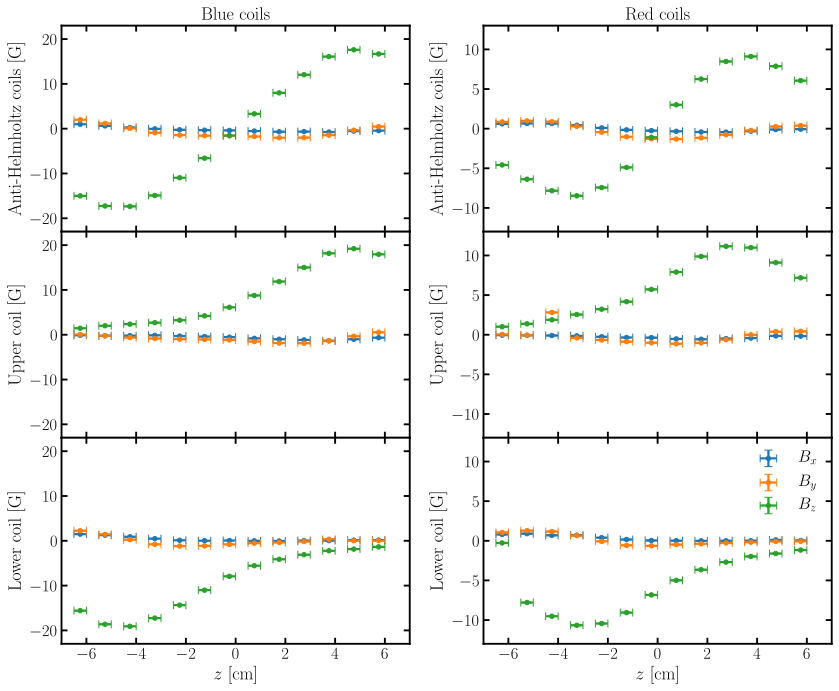
\includegraphics[keepaspectratio, width=\textwidth, height=\textheight]{experiment/mot_coils/mot_coil_fields.pdf}
	\caption{\label{fig:dual_mot_coil_fields}
		Blue MOT coil (left) and red MOT coil (right) magnetic fields measured along the $z$-axis on the test setup shown in \cref{fig:dual_mot_coils} with $I = \SI{4}{\ampere}$.
		The uncertainties are estimated to be $\delta_{z} = \pm \SI{2.5}{\cm}$ and $\delta_{B} = \pm \SI{0.05}{\gauss}$.
		The non-zero measured values of $B_x$ and $B_y$ suggest that the probe was slight off the $z$-axis.
		There also appears to be a slight systematic shift in zero-crossing of the anti-Helmholtz coils likely due to an uncertainty in determining the physical center of the coils.}
\end{figure}

**
It would have been nice to have an extra MOSFET switch on the blue MOT coils so that we'd be able to apply extremely large fields along the Z-axis such as e.g. Pedro's experiment Feshbach coils.
We're not too worried about not having this capability since ground-state strontium has no magnetic Feshbach resonances and the fact that we've observed a decrease MCP detection efficiencly we believe is due to the Lorentz force as the MCP is oriented along the X-axis.
**

\section{Laser Systems for Producing Cold and Ultracold Strontium Gases}

\Cref{fig:trapping_beams} gives an overview of the orientation of our various laser cooling and trapping beams.
\begin{sidewaysfigure}[htbp]
	\includesvg[keepaspectratio, width=\paperwidth, height=\paperheight]{experiment/laser_beams/trapping_beams.svg}
	\caption{\label{fig:trapping_beams}
		Simplified schematic of the various trapping and cooling lasers and the Rydberg excitation beams.}
\end{sidewaysfigure}

\subsection{\SI{461}{\nm} ``Blue'' Laser System}

The experiment currently has three blue diode lasers in a master-slave configuration which provide all the \SI{461}{\nm} power available for our experiment.
In a master-slave setup, a single (typically low-power) ``master'' external cavity diode laser (ECDL) is frequency stabilized relative to the atomic transition and is used to injection lock high-power ``slave'' lasers to amplify the laser power \cite{Shimada2013.RSI.84.063101, Hosoya2015.RSI.86.073110}.

Our current ECDL master laser\footnote{New Focus TLB-6802: a Littman-Metcalf external cavity diode laser (ECDL).} outputs about \SI{40}{\mW} and is locked relative to the $\nSLJ{5s^2}{1}{S}{0} \rightarrow \nSLJ{5s5p}{1}{P}{1}$ in a homebuilt strontium saturated absorption cell using Doppler-free saturated absorption spectroscopy.
The error signal is obtained by modulating the magnetic field around the saturated absorption cell and using circularly-polarized pump and probe beams.
Although this laser tunes relatively well and generally remains single-mode when tuning between the various isotopes, we have been very disappointed with output quality of the laser which has what appears to be a {Hermite-Gaussian TEM\tsub{00}} output mode **see Fig. XX). 
** INCLUDE BEAM PROFILER FIGURE **
Due to this poor output mode, a D-mirror was used to split the beam in to two nearly-Gaussian beams.
One of the beams is directed to a SMPM fiber which injection locks both our slave lasers whereas the other is currently unused.
After using the laser for about six years, the piezo tuning element died\footnote{The laser died after powering down and keying off the laser driver...} and the laser had to be sent back to New Focus for repairs.
During the repairs, we changed our setup so that the two slave lasers are injection locked from the output of a fiber so that we can easily change master lasers should this laser die again.
We also noticed some weird grounding issues with the TLB-6700 drivers New Focus sent us with the lasers\footnote{Similar issues were noticed by Jun Ye's group when I asked them if they have observed issues with the New Focus lasers.}.
Overall, we were not satisfied with New Focus' ECDL and their repair process and costs so much so that they only reduced the quoted repair cost\footnote{The piezo repair was going to cost 7500 with an additional 4000 for a new diode...} after we were ready to purchase a new \SI{461}{\nm} ECDL from either Toptica or MOGLabs\footnote{We ended up purchasing a \SI{461}{\nm} ECDL from Toptica but both companies provided quotes for NEW lasers, about 21k from MOGLabs and about 25k from Toptica but with about \SI{100}{\mW} of output power.}.

\begin{sidewaysfigure}[htbp]
	\centering
	\includesvg[keepaspectratio, width=\paperwidth, height=\paperheight]{experiment/blue_system/blue_system.svg}
	\caption{
		\label{fig:blue_system}
		Simplified diagram of the \SI{461}{\nm} laser system.}
\end{sidewaysfigure}

Light from the master laser injection locks two slave lasers\footnote{New Focus TLB-6802-IJ-D: a gratingless version of the TLB-6802 likely with a higher-power diode as well.}.
We have previously tried homebuilding our own \SI{461}{\nm} slave laser with can-opened blue diode\footnote{Nichia NDB4216E - a non-AR coated diode with about \SI{100}{\mW} of output power.} but found it to be unsatisfactory. 
We ended up going with two New Focus TLB-6802-IJ\footnote{From what we can tell, these are simply their standard TLB-6802 without the grating and probably using the Nichia NDB4216E non-AR coated diode which is specified to output about \SI{100}{\mW}.} both of which output about \SI{100}{\mW} of power.
The ``MOT'' slave is injection locked at the same frequency as the master laser and its power is split between the blue MOT, 2D collimator, and the imaging beam.
The injection beam for the ``Zeeman'' slave is first shifted by \SI{-535}{\MHz} relative to the master laser before injection locking the laser. This allows all the power out from the slave to be used for operating the Zeeman slower instead of taking a hit going through an AOM.

The entire \SI{461}{\nm} system is housed at far end of our table from the vacuum system and boxed in an opaque enclosure to contain the blue light, even a little of which can lead to heating our samples. 
Mechanical shutters\footnote{We use hard drive shutters as we've found them to be the most reliable.} are used to provide \SI{100}{\percent} extinction.
** Some details about our blue cooling system can be found in \cite{Camargo2015.MS, Ding2016.MS}. **

\subsection{\SI{481}{\nm} Repumping System}

Before moving on to the narrow line ``red'' MOT, the atoms in the metastable resevoir are dark to both the \SI{461}{\nm} and \SI{689}{\nm} cooling light and must be brought back to the ground state.

Our current \SI{481}{\nm} repumper system is shown in \cref{fig:repumper_system}. 
The \SI{481}{\nm} light is provided by a Toptica DL 100\footnote{The laser is equipped with a {LD-0488-0060-1} diode.} which outputs about ** \SI{10}{\mW} ** of power. 
For now, this laser is stabilized to a Doppler-broadened \Te{130}{2} line \cite{Wongwaitayakornkul2013.BS} which has a transition at \SI{20776.0886}{\per\cm} \cite{Cariou1980.Te2_Atlas} which is close to the $\nSLJ{5s5p}{3}{P}{2} \rightarrow \nSLJ{5p^2}{3}{P}{2}$ transition at \SI{20776.087}{\per\cm} \cite{Sansonetti2010.JPCRD.39.033103}.
Originally, when the lab was working with a single isotope, simply tuning the lock point to maximize repumping efficiency of the isotope of interest was good enough (typically \Sr{84} since it's the least abundant).
Now that we routinely work with multiple isotopes and mixtures, a free-space electro-optic modulator (EOM) was introducted to to add sidebands to the \SI{481}{\nm} light in order to address multiple isotopes and the hyperfine shift of \Sr{87}.
The hyperfine shift of the lower $\nSLJ{5s5p}{3}{P}{2}$ state is known \cite{Heider1977.PRA.16.1371} and cover the hyperfine shift of the upper $\nSLJ{5p^2}{3}{P}{2}$ doubly-excited is expected to be small **because of the lack of an {$s$-electron}\footnote{I.e., the magnetic dipole hyperfine contribution comes from the $\delta(r)$....} CHECK **.

\begin{figure}[htbp]
	\centering
	\includesvg[keepaspectratio, width=\textwidth, height=\textheight]{experiment/repumper_system/repumper_system.svg}
	\caption{
		\label{fig:repumper_system}
		Simplified diagram of our current \SI{481}{\nm} repumper laser system.
		A portion of the light form the \SI{481}{\nm} external cavity diode laser (ECDL) is used to lock to a Doppler-broadened \Te{130}{2} line in a cell heated to about \SI{555}{\celsius}.
		The rest of the light is sent through a free-space electro-optic modulator (EOM) at about \SI{565}{\MHz} which is used to apply sidebands to the light in order to address the various isotopes and hyperfine states.
		\SI{481}{\nm} light is delivered to the various experiments by multimode fibers.}
\end{figure}

In principle, it should be possible to lock to a hollow cathode lamp (HCL) due to collisions populating enough metastable atoms to perform spectroscopy on \cite{Norcia2016.RSI.87.023110}.
Instead of using an HCL, we plan on using a ``super lock'' \cite{Lindsay1991.RSI.62.1656, Jaffe1993.RSI.64.2475, Zhao1998.RSI.69.3737, Subhankar2019.RSI.90.043115} (see Appendix xxxx for future upgrade plans) since we already have a stable \SI{689}{\nm} reference laser (although we could also lock to a stabilized HeNe).
We also considered a lock to the wavemeter as in \cite{Couturier2018.RSI.89.043103} but ultimately decided against it as our wavemeter's accuracy is lacking, its sampling rate a bit too slow, and we needed the wavemeter for other tasks (e.g., finding Rydberg lines). 

\subsection{\SI{689}{\nm} ``Red'' Laser System}

Some details about our narrow line cooling system can be found in \cite{Ding2016.MS}.
The operation of the narrow line \SI{689}{\nm} ``red'' MOT can be found in \cite{Stellmer2013.PhD, Boyd2007.PhD, Ding2016.MS, Barker2016.PhD, Campbell2017.PhD}. 
Details of the \Sr{87} red MOT is particularly well described in \cite{Stellmer2013.PhD} and will not be reproduced here. 

\subsubsection{\SI{689}{\nm} Master Laser}

A single \SI{689}{\nm} Toptica DL pro ECDL serves as our master laser and is shared between the Rydberg and Neutral experiments. 
The laser is first locked to a homebuilt high-finesse Fabry-P{\'{e}}rot (FP) cavity\footnote{$F \gtrsim \num{2040}$ . Additional details can be found in \cite{Martinez2012.PhD}.} which is then locked to a heated strontium saturated absorption cell.
Since the $\SLJ{1}{S}{0} \rightarrow \SLJ{3}{P}{1}$ is very weak, the cell is relatively long to allow enough absorption to occur.
For most of the experiments described in this thesis, the red master laser was found to have a linewidth of about \SI{30}{\kHz}.
A diagram of the red master laser system is presented in \cite{Ding2016.MS}.
** More details of the \SI{689}{\nm} master laser system is provided in Jim's Ph.D. thesis. **
We recently purchased a ULE cavity from Stable Laser Systems (SLS). 
Some additional details in \cref{ssec:ULE_cavity}.

Due to the ease of building \SI{689}{\nm} slave lasers \cite{Ding2016.MS}, we only need a single \SI{689}{\nm} stabilized master laser system to run both the Rydberg and Neutral experiments. 
From the red master table, two fibers run to each experiment with light at the following frequencies:
\begin{itemize}
	\item $f_\text{master}$ --
		This light is locked to \SI{-82}{\MHz} of the $\nSLJ{5s^2}{1}{S}{0} \rightarrow \nSLJ{5s5p}{3}{P}{1}$ transition in \Sr{88}. 
	\item $f_\text{master} - \SI{1440.440}{\MHz}$ --
		This light is generated by passing the light directly out of the \SI{689}{\nm} master laser though a freespace gigahertz AOM before being sent to fibers to the Rydberg and Neutral experiments (instead of each experiment operating inefficient gigahertz AOMs to generate their own light for trapping \Sr{87}).
		This light is used to injection lock slave lasers for proudicing the \Sr{87} ``trap'' red MOT light.
\end{itemize}

We currently do not implement a fiber phase noise cancellation system \cite{Ma1994.OL.19.1777, Rauf2018.RSI.89.033103} so it's possible that the light at the slave lasers is broadened to ** kilohertz-levels ** over the \SI{25}{\meter} fibers delivering master light to the Rydberg experiment but it shouldn't be too difficult to implement in the future when necessary. 

\subsubsection{Rydberg Red Laser System}

Once the red light arrives on the Rydberg table, typically only about \SI{1}{\mW} is available so we use the master light to injection lock slave lasers to increase the available \SI{689}{\nm} power. 
\SI{689}{\nm} slave lasers are relatively easy to build and are detailed in \cite{Ding2016.MS}.
We currently use a rejected beam from the slave laser isolator to monitor the mode of the slave laser. 
In the future, I would instead use a stray reflection or beam sampler after the isolator as the current arrangement could lead to a small amount of light from the spectrum analyzer cavity getting back to the slave lasers (especially since we share the spectrum analyzer cavity with multiple slaves), possibly leading to instability issues. 

\Cref{fig:red_system} shows what the red MOT system looks like when set up for trapping any combination of isotopes. 
In practice, we don't always have all the red MOT AOMs lined up, typically only keeping the AOMs necessary for trapping the isotope(s) for a particular experiment while the other red MOT AOMs are used to generate various other beams (e.g., spectroscopy, ``blow away'', etc.).
\begin{sidewaysfigure}[htbp]
	\centering
	\includesvg[keepaspectratio, width=\paperwidth, height=\paperheight]{experiment/red_system/red_system.svg}
	\caption{\label{fig:red_system}Simplified diagram of the red MOT system (when everything is put together) for multi-isotope trapping. The master laser frequency is referenced to the $\nSLJ{5s^2}{1}{S}{0} \rightarrow \nSLJ{5s5p}{3}{P}{1}$ in \Sr{88}.}
\end{sidewaysfigure}
Without using a fiber combiner, we're able to devote a lot of power to the red MOT for each isotope, enabling us to use large red MOT beams. 
The drawbacks is that we're much more sensitive to misalignments and the ugly intensity profiles out of the diodes leads to strange red MOT shapes. 

We currently have three slave lasers which amplify the light from the red master. 
We found that fiber-coupling the injection beams made them much less sensitive to mechanical drifts and greatly increased the ease of switching the frequency of the slave laser by changing the source of the injection beam.

****
Image of \Sr{84} and \Sr{87} red MOTs.
****

Since the red MOT is only operated for a few hundred milliseconds, the zeroth-order from the red MOT AOMs also provide the light for various other purposes (e.g., spectroscopy, loss, etc.). 

**
Mention SWAP cooling? \cite{Norcia2018.NJP.20.023021, Bartolotta2018.PRA.98.023404, Muniz2018.arXiv.1806.00838, Snigirev2019.arXiv.1903.06435}.
**


\subsection{Optical Dipole Trap System}

Strontium in the ground $\nSLJ{5s^2}{1}{S}{0}$ state have a negligible magnetic moment meaning we cannot magnetically trap ground state atoms necessitating the use of optical traps. 
Our current high-power \SI{1064}{\nm} laser system is powered by a Nufern NuAMP SUB-1382 which amplifies a few milliwatts of \SI{1064}{\nm} seed light to about \SI{50}{\W}.
There are apparently ``tricks'' for making these lasers operate very quietly as used in quantum gas microscopes \cite{Mazurenko2017.PhD, Mazurenko2019.RSI.90.033101} but we have not done such modifications. 
Due to the high IR powers, we used fused silica optics whenever possible although we still have BK7 Brewster plates in the Thorlabs IO-5-1064-VHP isolator \cite{Mazurenko2017.PhD, Mazurenko2019.RSI.90.033101}.

We have used both free-space and fibered optical dipole traps but due to having to replace and realign the high-power IR lasers multiple times, we ended up sticking with the fibered systems due to them not losing alignment.
The drawback to the fibered ODT systems is that it's difficult to couple more than about \SI{10}{\W} through continuously without thermal effects degrading the coupling efficiency.
We get around this issue by only having the ODT on at high powers during the transfer from the red MOT before quickly moving on to the evaporation stage. 

We started with a free-spaced crossed-beam optical dipole trap (XODT) with waists of about $\SI{60}{\um} \times \SI{60}{\um}$. 
This trap was a bit tight but worked well for making \num{100000} BECs of \Sr{84}. 
We found that loading was improved if the trap was artificially widened by driving the AOM with three slightly different frequencies before turning the sideband frequencies down and evaporating \cite{Camargo2017.PhD}.
After going through three ODT lasers, we stuck with the sheet trap and vertical crossing trap because they were fiber coupled. 
Having the fiber-coulped sheet trap saved our ass as we've had to switch out the high-power laser multiple times (from the Coherent Verdi-IR, Nufern NuAmp, to IPG, back to Nufern NuAmp. 

For the high-power \SI{1064}{\nm} fibers, we've had good experiences using PMJ-A3AHPC,A3AHPC-1064-6/125-3AS-\textit{L}-1\footnote{These fibers are air-gapped and have an endcap on the ends which allows the beam to expand before entering/exiting the fiber, reducing hte power density. The adjustable fiber tip positions allow for optimization of coupling efficiency in to the fiber.} from OZ Optics. 

Our current main ODT is comprised of a single high-aspect ratio ``sheet'' trap with beam waists of about $\SI{28}{\um}$ (vertical) by $\SI{264}{\um}$ (horizontal), see \cref{fig:sheet_trap_profile}.
The design of the sheet trap was limited by sticking with $\SI{1}{\inch}$ optics and the relatively long distance to the atoms.
\begin{figure}[htbp]
	\centering
	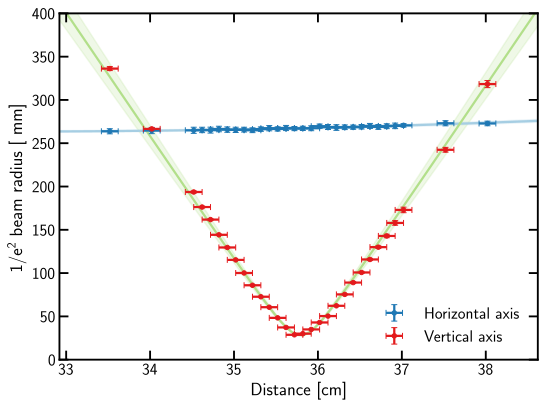
\includegraphics[keepaspectratio, width=4in]{experiment/odt_system/sheet_trap/sheet_trap_profile/sheet_profile.pdf}
	\caption{
		\label{fig:sheet_trap_profile}
		Beam profile of the sheet trap from which we fit to obtain the beam waists.
		For the vertical waist: $w = \SI{28.0+-1.0}{\um}$, $z_{0} = \SI{35.795+-0.009}{\cm}$, and $M^2 = \num{1.18+-0.04}$.
		For the horizontal waist: $w = \SI{263.5+-0.9}{\um}$, $z_{0} = \SI{32.3+-0.4}{\cm}$, and $M^2 = \num{1.0}$.
		Distances are measured from the end of the cage system assuming $\pm \SI{1}{\mm}$ uncertainty.}
\end{figure}

To increase the horizontal trap frequency, we also implemented a circular ODT beam which intersects the sheet trap at a near vertical angle.
The measured beam profile of the vertical trap is shown in \cref{fig:vertical_trap_profile}.
\begin{figure}[htbp]
	\centering
	\includegraphics[keepaspectratio, width=4in]{experiment/odt_system/vertical_trap/vertical_trap_profile/vertical_profile.pdf}
	\caption{
		\label{fig:vertical_trap_profile}
		Beam profile of the vertical trap from which we fit to obtain the beam waists.
		An assumed $\pm \SI{1}{\mm}$ uncertainty in the measured distance and $\pm \SI{5}{\um}$ uncertainty in the measured waist size.}
\end{figure}
We attempted to circularly polarized the vertical ODT so that we would be able to minimize the differential shifts and enable cooling in to the ODT \cite{Ido2003.PRL.91.053001, Stellmer2013.PRA.87.013611} but we didn't observe any improvement in loading the ODT.
This lack of improvement is probably due to our $\SI{689}{\nm}$ laser system being a bit too broad to take advantage of this.

\section{Making and Detecting Rydberg Atoms}

Now that we have an ultracold sample of strontium, we use a $\SI{320}{\nm}$ UV laser system to excite them to Rydberg atoms via the two-photon transition from the intermediate $\nSLJ{5s5p}{3}{P}{1}$ state.
The electric field system and charged particle detection will be detailed in Joe Whalen's upcoming Ph.D. thesis so they will only be briefly covered here. 

% \begin{sidewaysfigure}[htbp]
	% \includesvg[keepaspectratio, width=\paperwidth, height=\paperheight]{experiment/laser_beams/rydberg_beams.svg}
	% \caption{\label{fig:rydberg_beams}
		% Diagram of the various Rydberg excitation beams.}
% \end{sidewaysfigure}

\subsection{$\SI{320}{\nm}$ UV Laser System}

Strontium Rydberg atoms are produced using a two-photon transtion where a $\SI{689}{\nm}$ and a $\SI{320}{\nm}$ photon drives atoms from the $\nSLJ{5s^2}{1}{S}{0}$ ground state to either a $\nSLJ{5sns}{3}{S}{1}$ or $\nSLJ{5snd}{3}{D}{J}$ states. 

Generation of the $\SI{320}{\nm}$ radiation starts with a tunable, narrow linewidth $\SI{1064}{\nm}$ seed laser which is amplified to about $\SI{7.5}{\watt}$ by a fiber amplifier\footnote{IPG Photonics YAR-15K-1064-LP-SF ytterbium fiber amplifier.}.
We currently have two $\SI{1064}{\nm}$ seed lasers in the lab and choose the laser based on the experiment
\begin{itemize}
	\item Koheras Basik BMY10PztSPm, KOH2038 --
		The narrowest $\SI{640}{\nm}$ lines we've seem with this seed are around ** $\SI{1}{\MHz}$ **, likely limited by the slow feedback bandwidth of the piezo element, but it's capable of tuning multiple GHz so it's preferred for experiments requiring large tuning.
	\item NP Photonics Rock RFLM-50-3-1064.53-1-S-0 --
		The feedback bandwidth of this laser is quite a bit better than the Koheras with ** $\SI{250}{\kHz}$ ** being the narrowest features we've observed.
		Although the feedback bandwidth results with a narrow $\SI{640}{\nm}$ linewith, it's more difficult to continuously tune large ranges. 
\end{itemize}
The output of the fiber amplifier pumps a Lockheed Martin Aculight Argos Model 2400 CW optical parametric oscillator (OPO) modified with a sum frequency generation stage. 
Similar to the setup described in \cite{Mieth2014.OE.22.11182}, OPO-SFG is achieved by replacing the standard OPO crystal with periodically poled, magnesium-oxide-doped lithium niobate crystal ({MgO:PPLN}) where the first section is poled for OPO and second section is poled for SFG.
The cavity dichroics were also replaced.
The OPO section uses the $\lambda_{\text{P}} = \SI{1.064}{\um}$ pump to generate $\lambda_{\text{S}} = \SI{1.6}{\um}$ and $\lambda_{\text{I}} = \SI{3.2}{\um}$ light.
The SFG section then combines the $\lambda_{\text{S}} = \SI{1.6}{\um}$ with another $\lambda_{\text{P}} = \SI{1.064}{\um}$ to produce $\lambda_{\text{SFG}} = \SI{640}{\nm}$.

As mentioned in \cite{DeSalvo2015.PhD}, temperature tuning of the crystal is required for efficient $\SI{640}{\nm}$ generation but the Argos system was only designed for heating.
A workaround was developed where a water-cooling block was attached to the outside of the OPO cavity housing to lower the temperature enough to where the Argos' internal heater is capable stabilizing the temperature (see \cref{fig:argos_opo	}).
With this addition, we typically get about ** \SIrange[range-phrase=-]{1}{1.5}{\watt} ** of $\SI{640}{\nm}$.
\begin{figure}[htbp]
	\centering
	\includesvg[keepaspectratio, width=\textwidth, height=\textheight]{experiment/uv_system/argos_opo/argos_opo.svg}
	\caption{
		\label{fig:argos_opo}
		Picture of the Lockheed Martin Aculight Argos Model 2400 CW OPO with the custom water-cooling block attached to the cavity housing.
		The current tubing on the cooling block is a bit too stiff to bend enough to put the laser cover on.}
\end{figure}

Stabilization of the $\SI{640}{\nm}$ laser frequency is accomplished with a transfer cavity lock \cite{Riedle1994.RSI.65.42, Bohlouli2006.RSI.77.093105, Leopold2016.APB.122.236} where the length of a tunable optical cavity is first stabilized to the $\SI{689}{\nm}$ laser (which itself is stabilized to an atomic reference) and then stabilizing the $\SI{640}{\nm}$ to the cavity.
Some of the details of our transfer cavity are documented in \cite{Zha2013.BS}.
Briefly, our transfer cavity is constructed from an Invar body with the cavity mirrors attached to a piezoelectric (PZT) stack on each end. 
The PZT on one end is used to stabilize the cavity length to the $\SI{689}{\nm}$ laser while the other end provides a tunable ``offset'' which we can use to lock to different FSRs of the transfer cavity.
Pound-Drever-Hall (PDH) \cite{Drever1983.APB.31.97, Black2001.AJP.69.79} is used to lock the cavity length to the $\SI{689}{\nm}$ reference and to lock the $\SI{640}{\nm}$ to the cavity.
The optical layout at the transfer cavtiy is shown in \cref{fig:transfer_cavity}.
\begin{figure}[htbp]
	\centering
	\includesvg[keepaspectratio, width=\textwidth, height=\textheight]{experiment/uv_system/transfer_cavity.svg}
	\caption{
		\label{fig:transfer_cavity}
		Simplified diagram of our transfer cavity setup.
		** NEED TO FINISH **.}
\end{figure}
Tunability is achieved with a broadband fiber EOM (fEOM) between the $\SI{640}{\nm}$ laser output and the transfer cavity. 
The PDH error signal is fedback to the $\SI{1064}{\nm}$ seed laser.
Although we have not done a full characterization of the linewidth of the $\SI{640}{\nm}$ laser, the narrowest Rydberg lines we have seen are about ** $\SI{150}{\kHz}$ in $\SI{640}{\nm}$** which can be considered an upper bound on the laser's short-term stability.
Longer-term stability isn't as good where we have seen drifts of about ** $\SI{500}{\kHz}$ ** when scanning over the same Rydberg (molecule) lines.
With the recent acquisition of a ULE cavity (see \cref{ap:upgrades}), we plan to eliminate the transfer cavity in favor of locking the $\SI{640}{\nm}$ directly to the ULE cavity with a setup similar to the one presented in \cite{Gregory2015.NJP.17.055006}.

Now that we have a tunable and stabilized source of $\SI{640}{\nm}$, the output from the OPO is then coupled in to a commercial Toptica second-harmonic generation (SHG) pro system which produces doubles the $\SI{640}{\nm}$ to $\SI{320}{\nm}$.
When well-tuned, the system is capable of outputting  ** $> \SI{500}{\milli\W}$ of power but it tends to degrade over time.
Our typical operating powers are closer to about $\SI{100}{\milli\W}$.
\begin{figure}[htbp]
	\centering
	\includesvg[keepaspectratio, width=\textwidth, height=\textheight]{experiment/uv_system/toptica_shg_pro/toptica_shg_pro-cavity.svg}
	\caption{
		\label{fig:toptica_shg_pro-cavity}
		Picture of the Toptica SHG pro bow tie doubling cavity. 
		The normally-sealed SHG cavity was opened up when realigning the $\SI{640}{\nm}$ to the cavity.}
\end{figure}

\subsection{Electric Field System}

Due to the extreme ${n}^{7}$ scaling of polarizability \cite{Gallagher1988.RPP.51.143, Gallagher1994.RydbergAtoms}, Rydberg atoms are extremely sensitive to electric fields. 
To mitigate stray electric fields at the location of the atoms as well as to provide the capability for trimming residual electric fields and perform selective field ionization (SFI), we installed in-vacuum electric field plates. 
The electric field plate system was designed by Francisco Camargo and additional details his Ph.D. thesis \cite{Camargo2017.PhD} and the design follows similar ones described in \cite{Millen2011.PhD, Low2012.JPB.45.113001} using a split-ring electrode geometry with four quadrant electrodes above and four quadrant electrodes below the center of the chamber (i.e., where the atoms are). 
The split-ring electrodes and in vacuum wires are made from oxygen-free high conductivity (OFHC) copper with stainless steel making up the supporting scaffold, Einzel lens, and guiding plates. 
All parts were polished by hand before being sent off to be electropolished. 

** Stuff about the scaffold and copper electric field plates. SIMION simulations? **

\begin{figure}[htbp]
	\centering
	\includesvg[keepaspectratio, width=\textwidth, height=\textheight]{experiment/electric_field_system/electric_field_system-CAD.svg}
	\caption{
		\label{fig:electric_field_system-CAD}
		CAD renderings of the electric field plates with most of the supporting scaffold removed.
		Blue spheres represent the sapphire spacers used to isolate the high-voltage components from the grounded support structure.
		(Left) Top view of the eight electric field plates, Einzel lens, guiding plates, and MCP.
		The eleven \SI{10}{\kV} SHV feedthroughs are numbered clockwise.
		Red circles highlight the locations of the feedthroughs which are partially obstructed from view by the bottom scaffold plate.
		(Right) The electrodes are numbered corresponding to the feedthrough on the bottm flange.}
\end{figure}

We currently have a (limited) ability to change how the electric field plates are ramped depending on whether want want to detect electrons or ions, and whether we want to perform selective field ionization (SFI). 
Most of the work presented in this thesis involves detecting electrons and just using the integrating the SFI spectra (i.e., we simply count all the electrons). 
When taking data, we monitor the SFI spectra to make sure that the entire Rydberg signal(s) is captured but the data analysis simply uses the total Rydberg electron counts. 
An example SFI spectrum is shown in \cref{fig:example_mcs_signal}. 

\begin{figure}[htbp]
	\centering
	\includesvg[keepaspectratio, width=\textwidth, height=\textheight]{experiment/electric_field_system/electric_field_system-real.svg}
	\caption{
		\label{fig:electric_field_system-real}
		(Left) Overview of the actual electric field system mounted on the bottom flange of main chamber. 
		Connections between the feedthroughs and the electric field plates are made with OFHC wires and insulated from the grounded supporting scaffold wtih ceramic fish spine beads. 
		Beryllium-copper inline barrel connectors with two cross-screws attach the wires to the feedthroughs.
		(Right) Close up of the eight electric field plates, Einzel lens, and guiding plates.
		The sapphire spheres (red or clear) which isolate the high-voltage parts from the grounded scaffold structure are also visible.}
\end{figure}

Working at high-$n$, Soumya was able to trim electric fields to better than ** xxxx V/cm ** when taking spectra at $n=160$.
We should be able to improve our electric field zeroing a bit more if we're more careful with biases on the SFI HV switches but extremely accurate switching would likely require going to a different design (** e.g. Tilman Pfau's box **).
For now, the electric field system is sufficient for our purposes. 

\subsection{Charged Particle Detection}

One of the major aspects which separates our experiment from most other neutral atom experiments is the ability to detect charged particles. 
Some of the previous work with strontium Rydberg experiments was carried out in the Neutral appratus but since they lacked the ability to detect charged particles, they had to resort to detecting atom loss in absorption images \cite{DeSalvo2015.PRA.92.031403, DeSalvo2016.PRA.93.022709, Aman2016.PRA.93.043425}.
Our system was designed from the beginning to be able to detect charged particles which we've found to be incredibly sensitive with teh ability to detect signals spanning several orders of magnitude \cite{Camargo2018.PRL.120.083401}.
** Since Joe will be detailing the electric field ionization and detection system in his upcoming Ph.D. thesis, only the major detials are included here for completeness. **

An overview of how our charted particle detection system works is shown in \cref{fig:charged_particle_detection}.
The following procedure explains how we detect electrons as that's what we primarily work with but we have configured our system to detection ions instead.
** CHECK !! ** After performing a Rydberg excitation on a sample, we typically apply a symmetric field ramp where the plates closer (further) from the MCP are ramped to positive (negative) high-voltage to push electrons towards the MCP. 
The length of the cables from the HV switch\footnote{Willamette High Voltage PHVSW-005.} to each of the feedthroughs are about the same length to keep the capacitance approximately equal.
\begin{figure}[htbp]
	\centering
	\includesvg[keepaspectratio, width=\textwidth, height=\textheight]{experiment/mcp/charged_particle_detection.svg}
	\caption{
		\label{fig:charged_particle_detection}
		** PLACEHOLDER FIGURE **.
		Charged particle detection system.}
\end{figure}
We adjust the HV supplies for the electric field plate ramps depending on which principal quantum number ($n$) of the Rydberg state we are exciting. 
Due to the cable capacitance, this also affects the ramp rate of the applied electric field but it doesn't significantly affect our data since we're primarily interested in the integrated SFI spectrum.

Charged particles are detected with an MCP\footnote{Photonis Advanced Performance Detector (APD) 2 miniTOF. It's important to note that we purchased the version with PEEK components so care must be taken when performing a bake-out.} where the front plate is kept fixed at $\SI{200}{\V}$ while the back of the MCP is fixed at $\SI{2650}{\V}$.
The MCP is mounted to a $\SI{2.75}{\inch}$ flange with four HV feedthroughs with ceramic insulation.
\begin{figure}[htbp]
	\centering
	\includesvg[keepaspectratio, width=\textwidth, height=\textheight]{experiment/mcp/mcp.svg}
	\caption{
		\label{fig:mcp}
		Pictures of the MCP mounted to a $\SI{2.75}{\inch}$ flange with high-voltage feedthroughs. 
		Like the electric field plates, connections are made with beryllium-copper inline barrel connectors.
		Ceramic washers were placed between the screws to act as a spacer to keep the connections from touching eachother and the main vacuum chamber.}
\end{figure}
Currently, the MCP's output is first connected to a preamplifier\footnote{Stanford Research Systems SR445.} which is then fed in to an RF amplifier\footnote{ZFL-500LN.} to remove DC offsets before going to the MCS\footnote{FAST ComTec GmbH MCA-3 P7882.}. 
An example Rydberg signal from the MCS is shown in \cref{fig:example_mcs_signal}.
\begin{figure}[htbp]
	\centering
	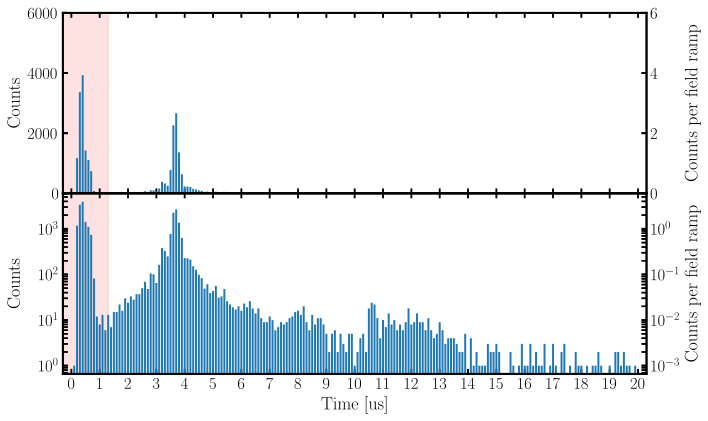
\includegraphics[keepaspectratio, width=\textwidth, height=\textheight]{experiment/mcp/example_mcs_signal/example_mcs_signal.pdf}
	\caption{
		\label{fig:example_mcs_signal}
		Example MCS signal from the $\nSLJf{5s38s}{3}{S}{1}{\flatfrac{11}{2}}$ Rydberg line in \Sr{87} for a single detuning in (top) linear scale and (bottom) log scale.
		There are $\num{200}$ $\SI{100}{\ns}$ bins with the electric field ramp starting at $t = \SI{0}{\ns}$.
		To increase signal, we perform multiple excitation-detection sequences and sum the resulting counts bin-by-bin. 
		Dividing by the total number of loops gives the counts per bin per loop ($\num{1000}$ loops were used in the data above).
		The MCS detects a large ``kick'' for first several bins (shaded region) so the data in those bins (shaded region) are dropped before proceeding with the analysis.}
\end{figure}

As seen in \cref{fig:mcp_saturation}, MCPs are known to ``saturate'' and become non-linear as the count rate increases.
This non-linearity is important to characterize so that we know when the signal is in the linear regime and when we need to start taking in to account the non-linearity in detection efficiency. 
\begin{figure}[htbp]
	\centering
	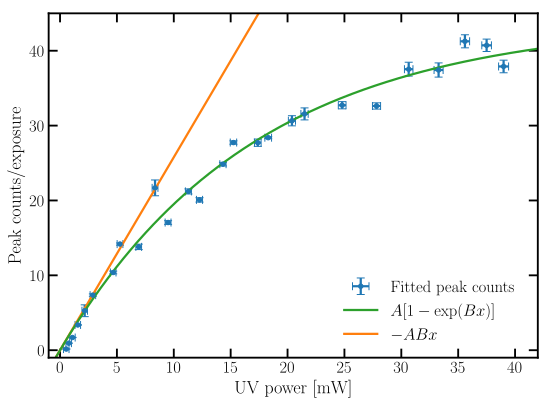
\includegraphics[keepaspectratio, width=4in]{experiment/mcp/mcp_saturation/20190327-Complete_data_set/mcp-counts_vs_uv_power.pdf}
	\caption{
		\label{fig:mcp_saturation}
		Peak integrated SFI spectrum per $\SI{10}{\us}$ exposure vs. UV excitation power exciting to the $\nSLJf{5s33s}{3}{S}{1}{\flatfrac{11}{2}}$ state of \Sr{87} in a $B_{x} \approx \SI{1.1}{\gauss}$ bias field (\SI{689}{\nm} power kept constant).
		The peak counts were obtained by fitting to the Zeeman-split spectra and extracting the height of the $m_{F} = \flatfrac{11}{2}$ line.
		Since $\num{1000}$ $\SI{10}{\us}$ exposures were used for each frequency point, the fitted peak counts was divided by $\num{1000}$ to obtain the counts per exposure.
		Fitting to the empirical model $A \qty[1 - \exp(B x)]$ results with the coefficients $A = \num{44.0+-1.7}$ and $B = \num{-0.059+-0.005}$.}
\end{figure}
Performing a fit to the empirical model
\begin{equation}
	y = A \qty[1-\exp(B x)]
\end{equation}
allows us to determine the constants $A$ and $B$ so that we can extract correct for undercounting regardless of whether our signal is in the linear-regime or not.